\documentclass[t]{beamer} % [t] pomeni poravnavo na vrh slida

% \usepackage{etex} % vključi ta paket, če ti javi napako, da imaš naloženih preveč paketov.

% standardni paketi
\usepackage[slovene]{babel}
\usepackage[T1]{fontenc}
\usepackage[utf8]{inputenc}
\usepackage{amssymb}
\usepackage{amsmath}
\usepackage{mathrsfs}
\usepackage{graphicx}
\usepackage{import}
\graphicspath{ {./slike/} }



% paket, ki ga rabimo za risanje
\usepackage{pgf,tikz,pgfplots}
\usetikzlibrary{arrows}
\usepackage{lmodern}                            % to get rid of font warnings
\renewcommand\textbullet{\ensuremath{\bullet}}  % to get rid of font warnings
\usepackage{verbatim, subcaption}
\usepackage{pgfplots}
\usetikzlibrary{arrows.meta, calc, positioning, automata}
% podatki
\title{Izrek o invarianci odprtih množic}
\author{Tom Gornik}
\institute{mentor: izr.\ prof.\ dr.\ Jaka Smrekar}

% tvoj izbran stil predstavitve
\usetheme{Singapore}
\usecolortheme{crane}
\beamertemplatenavigationsymbolsempty
% \setbeamertemplate{footline}{}            % pri nekaterih temah je potrebno odstraniti
% \setbeamertemplate{navigation symbols}{}  % nogo, v tem primeru to odkomentiraj

%  ukaz za počrnitev enega slida. Nariše črn pravokotnik višine #1 na dno.
\newcommand{\fillblack}[1]{
\begin{tikzpicture}[remember picture, overlay]
    \node [shift={(0 cm,0cm)}]  at (current page.south west)
        {%
        \begin{tikzpicture}[remember picture, overlay] at (current page.south west)
            \draw [fill=black] (0, 0) -- (0,#1 \paperheight) --
                              (\paperwidth,#1 \paperheight) -- (\paperwidth,0) -- cycle ;
        \end{tikzpicture}
        };
        \draw (current page.north west) rectangle (current page.south east);
\end{tikzpicture}
}

% Projektor, ki sveti na tablo je zoprn, ker zavzema prostor za pisanje.
% Praktična rešitev je, da se platno spusti samo do table, spodnji del
% predstavitve pa naredimo popolnoma črn. Tako projektor na tablo ne projecira
% svetlobe in je pisanje nemoteno s strani predstavitve, ki je cela nad tablo.

% Za to da dobite spodaj zatemnjen slide, je potrebno na konec frame-a dodati
% ukaz \fillblack{delež}, kjer je delež številka med 0 in 1, ki pove, kakšen
% delež slida želite imeti zapolnjen s črnim pravokotnikom. Spodaj so 4 slidi,
% ki imajo začrnjenih: 33%, 50%, 33% in 20%.  Za šolske table v 2.02 in 2.03 je
% 33% ravno prav, da lahko pišete po celi tabli.

% Črni pravokotnik ne zavzema prostora na slidu -- preprosto nariše se čez
% spodnjo tretjino (ali kolikor pač želite). To pomeni, da se pokrijve tudi ves
% tekst spodaj. Za to je na začetku dokumenta tudi nastavljena vertikalna
% poravnava na ``zgoraj'', z razliko od običajne sredinske (to je tisti [t]).
% Tako se ves tekst obdrži na vidnem delu slida, dokler je to možno. Tretji
% slide spodaj demonstrira, kaj se zgodi v primeru preveč besedila.

% Kod demonstrira zadnji slide, je vseeno, kjer napišemo ukaz, toda ponavadi ga
% napišemo na dnu, da se izognemo morebitnim nevšečnostim ali neželenemu
% spacingu. Pri nekaterih temah se izriše tudi noga, ki se izriše na koncu
% slida, torej po tem ko je naš pravokotnik že narisan, kar zna biti moteče.
% To se na primer zgodi tudi pri standardni temi Warsaw. Rešitev je, da nogo
% odstranimo (saj bi bila itak prekrita). V preambuli so zakomentirani ukazi,
% kako to naredimo.

\begin{document}

\begin{frame}
  \maketitle
\end{frame}



\begin{frame}{Zakaj izrek o invarianci odprtih množic?}
\begin{itemize}
\item Presenetljivo težko dokazati,
\item<2>[] \includegraphics[width=7cm]{peano_curve.jpg}
\end{itemize}
\end{frame}

\begin{frame}{Zakaj izrek o invarianci odprtih množic?}
\begin{itemize}
\item lepa slika dokaza.
\item<2>[] \includegraphics[width=8.5cm]{glavna_slika.pdf}
\end{itemize}
\end{frame}


\begin{frame}
\frametitle{Izrek o invarianci odprtih množic}
\begin{block}{Izrek o invarianci odprtih množic}
Naj bo $U$ odprta množica v evklidskem prostoru $\mathbb{R}^n$ in naj bo $h : U \rightarrow \mathbb{R}^n$ zvezna injekcija. Potem je tudi slika $h(U)$ odprta množica v $\mathbb{R}^n$
\end{block}
\end{frame}

\begin{frame}
\frametitle{Izrek o invarianci odprtih množic}
\begin{figure}
\begin{tikzpicture}
% ####################   elastika    ####################
\draw plot [smooth cycle, tension = 1.2] coordinates {(-1, 2.2) (-2, 0) (-1.3, -3) (1, -2.5) (1.8, 0.9)};
\draw plot [smooth cycle, tension = 1] coordinates {(7, 2.2) (5.3, 0) (6.7, -3) (7.8, -2.5) (8, 0.9)};
\draw (-1.5, 1.8) node {$U$};
\draw (7, 1.8) node {$h(U)$};
\draw[->] (2.5, 0) -- (4.5,0);
\draw (3.5, 0.5) node {$h$};
\end{tikzpicture}
\end{figure}
\end{frame}

\begin{frame}
\frametitle{Izrek o invarianci odprtih množic}
\begin{figure}
\begin{tikzpicture}
% ####################   elastika    ####################
\draw plot [smooth cycle, tension = 1.2] coordinates {(-1, 2.2) (-2, 0) (-1.3, -3) (1, -2.5) (1.8, 0.9)};
\draw plot [smooth cycle, tension = 1] coordinates {(7, 2.2) (5.3, 0) (6.7, -3) (7.8, -2.5) (8, 0.9)};
\draw (-1.5, 1.8) node {$U$};
\draw (7, 1.8) node {$h(U)$};
\draw[->] (2.5, 0) -- (4.5,0);
\draw (3.5, 0.5) node {$h$};
\filldraw[black] (1, -1) circle (1pt) node[anchor=north west] {$x$};
\filldraw[black] (6, 1) circle (1pt) node[anchor=north west] {$h(x)$};
\end{tikzpicture}
\end{figure}
\end{frame}

\begin{frame}
\frametitle{Izrek o invarianci odprtih množic}
\begin{figure}
\begin{tikzpicture}
% ####################   elastika    ####################
\draw plot [smooth cycle, tension = 1.2] coordinates {(-1, 2.2) (-2, 0) (-1.3, -3) (1, -2.5) (1.8, 0.9)};
\draw plot [smooth cycle, tension = 1] coordinates {(7, 2.2) (5.3, 0) (6.7, -3) (7.8, -2.5) (8, 0.9)};
\draw (-1.5, 1.8) node {$U$};
\draw (7, 1.8) node {$h(U)$};
\draw[->] (2.5, 0) -- (4.5,0);
\draw (3.5, 0.5) node {$h$};
\filldraw[black] (1, -1) circle (1pt) node[anchor=north west] {$0$};
\filldraw[black] (6, 1) circle (1pt) node[anchor=north west] {$h(0) = b$};
\end{tikzpicture}
\end{figure}
\end{frame}

\begin{frame}
\frametitle{Izrek o invarianci odprtih množic}
\begin{figure}
\begin{tikzpicture}
% ####################   elastika    ####################
\draw plot [smooth cycle, tension = 1.2] coordinates {(-1, 2.2) (-2, 0) (-1.3, -3) (1, -2.5) (1.8, 0.9)};
\draw plot [smooth cycle, tension = 1] coordinates {(7, 2.2) (5.3, 0) (6.7, -3) (7.8, -2.5) (8, 0.9)};
\draw (-1.5, 1.8) node {$U$};
\draw (7, 1.8) node {$h(U)$};
\filldraw[black] (1, -1) circle (1pt) node[anchor=north west] {$0$};
\filldraw[black] (6, 1) circle (1pt) node[anchor=north west] {$h(0) = b$};
\draw[->] (2.5, 0) -- (4.5,0);
\draw (3.5, 0.5) node {$h$};
\draw (0.5, -1.5) rectangle (1.5, -0.5);
\draw (1, -0.3) node {$\mathbb{I}^n$};
\end{tikzpicture}
\end{figure}
\end{frame}



\begin{frame}
\frametitle{Izrek o invarianci odprtih množic}
\begin{figure}[h!]
\begin{tikzpicture}[scale=0.78]
% ###############          prva slika          ###############
		\draw (-5.9, 1.8) rectangle (-3.3, 4.2);
		\filldraw[red] (-4.6, 3) circle (1.5pt) node[black, above right=-0.7mm] {$0$};	
		 \draw (-3.6, 3.85) node {$\mathbb{I}^n$};
		
% ###############          druga slika          ###############
		\draw plot [smooth cycle, tension = 0.3] coordinates {(2.3, 1.45) (5.2, 1.5) (5.25, 4.65) (4.25, 4.7) (4.2, 2.5) (3.15, 2.5) (3.7, 4.2) (3.5, 4.4) (2.8,3.7)  (2.5, 3.2) (2.3, 2.5)};
		\draw (4.6, 2) node {$h(\mathbb{I}^n)$};
	
% ###############          tretja slika          ###############
		
		\draw[white] (4.8, -4) node {$X$}; 
		
	
	% ###############          puščice          ###############
		\draw [black, line width=1.2pt, -Stealth] (-1.7,3) -- (1.2,3);
		\draw (-0.4, 3.6) node {$h$};
	\end{tikzpicture}
\end{figure}
\end{frame}

\begin{frame}
\frametitle{Izrek o invarianci odprtih množic}
\begin{figure}[h!]
\begin{tikzpicture}[scale=0.78]
% ###############          prva slika          ###############
		\draw (-5.9, 1.8) rectangle (-3.3, 4.2);
		\filldraw[red] (-4.6, 3) circle (1.5pt) node[black, above right=-0.7mm] {$0$};	
		 \draw (-3.6, 3.85) node {$\mathbb{I}^n$};
		
% ###############          druga slika          ###############
		\draw plot [smooth cycle, tension = 0.3] coordinates {(2.3, 1.45) (5.2, 1.5) (5.25, 4.65) (4.25, 4.7) (4.2, 2.5) (3.15, 2.5) (3.7, 4.2) (3.5, 4.4) (2.8,3.7)  (2.5, 3.2) (2.3, 2.5)};
		\filldraw[red] (4.21, 4.2) circle (1.5pt) node[black, right=-0.7mm] {$b$};
		\draw (4.6, 2) node {$h(\mathbb{I}^n)$};
	
% ###############          tretja slika          ###############
		\draw[white] (4.8, -4) node {$X$}; 
		
	% ###############          četrta slika          ###############
		
	% ###############          puščice          ###############
		\draw [black, line width=1.2pt, -Stealth] (-1.7,3) -- (1.2,3);
		\draw (-0.4, 3.6) node {$h$};
	\end{tikzpicture}
\end{figure}
\end{frame}

\begin{frame}
\frametitle{Izrek o invarianci odprtih množic}
\begin{figure}[h!]
\begin{tikzpicture}[scale=0.78]
% ###############          prva slika          ###############
		\draw (-5.9, 1.8) rectangle (-3.3, 4.2);
		\filldraw[red] (-4.6, 3) circle (1.5pt) node[black, above right=-0.7mm] {$0$};	
		 \draw (-3.6, 3.85) node {$\mathbb{I}^n$};
		
% ###############          druga slika          ###############
		\draw plot [smooth cycle, tension = 0.3] coordinates {(2.3, 1.45) (5.2, 1.5) (5.25, 4.65) (4.25, 4.7) (4.2, 2.5) (3.15, 2.5) (3.7, 4.2) (3.5, 4.4) (2.8,3.7)  (2.5, 3.2) (2.3, 2.5)};
		\filldraw[red] (4.21, 4.2) circle (1.5pt) node[black, right=-0.7mm] {$b$};
		\draw (4.6, 2) node {$h(\mathbb{I}^n)$};
		\draw[black] (4.21, 4.2) circle (42pt);
		\draw (6.25, 5.25) node {$B(b, 2 \delta)$};
	
% ###############          tretja slika          ###############
		\draw[white] (4.8, -4) node {$X$}; 
		
	% ###############          četrta slika          ###############
		
	% ###############          puščice          ###############
		\draw [black, line width=1.2pt, -Stealth] (-1.7,3) -- (1.2,3);
		\draw (-0.4, 3.6) node {$h$};
	\end{tikzpicture}
\end{figure}
\end{frame}

\begin{frame}
\frametitle{Izrek o invarianci odprtih množic}
\begin{figure}[h!]
\begin{tikzpicture}[scale=0.78]
% ###############          prva slika          ###############
		\draw (-5.9, 1.8) rectangle (-3.3, 4.2);
		\filldraw[red] (-4.6, 3) circle (1.5pt) node[black, above right=-0.7mm] {$0$};	
		 \draw (-3.6, 3.85) node {$\mathbb{I}^n$};
		
% ###############          druga slika          ###############
		\draw plot [smooth cycle, tension = 0.3] coordinates {(2.3, 1.45) (5.2, 1.5) (5.25, 4.65) (4.25, 4.7) (4.2, 2.5) (3.15, 2.5) (3.7, 4.2) (3.5, 4.4) (2.8,3.7)  (2.5, 3.2) (2.3, 2.5)};
		\filldraw[red] (4.21, 4.2) circle (1.5pt) node[black, right=-0.7mm] {$b$};
		\filldraw[black] (3.9, 4) circle (2pt) node[black, below =-0.1mm]{$c$};
		\draw (4.6, 2) node {$h(\mathbb{I}^n)$};
		\draw[black] (4.21, 4.2) circle (42pt);
		\draw (6.25, 5.25) node {$B(b, 2 \delta)$};
	
% ###############          tretja slika          ###############
		\draw[white] (4.8, -4) node {$X$}; 
		
	% ###############          četrta slika          ###############
		
	% ###############          puščice          ###############
		\draw [black, line width=1.2pt, -Stealth] (-1.7,3) -- (1.2,3);
		\draw (-0.4, 3.6) node {$h$};
	\end{tikzpicture}
\end{figure}
\end{frame}

\begin{frame}
\frametitle{Izrek o invarianci odprtih množic}
\begin{figure}[h!]
\begin{tikzpicture}[scale=0.78]
% ###############          prva slika          ###############
		\draw (-5.9, 1.8) rectangle (-3.3, 4.2);
		\filldraw[red] (-4.6, 3) circle (1.5pt) node[black, above right=-0.7mm] {$0$};	
		 \draw (-3.6, 3.85) node {$\mathbb{I}^n$};
		
% ###############          druga slika          ###############
		\draw plot [smooth cycle, tension = 0.3] coordinates {(2.3, 1.45) (5.2, 1.5) (5.25, 4.65) (4.25, 4.7) (4.2, 2.5) (3.15, 2.5) (3.7, 4.2) (3.5, 4.4) (2.8,3.7)  (2.5, 3.2) (2.3, 2.5)};
		\filldraw[red] (4.21, 4.2) circle (1.5pt) node[black, right=-0.7mm] {$b$};
		\filldraw[black] (3.9, 4) circle (2pt) node[black, below =-0.1mm]{$c$};
		\draw (4.6, 2) node {$h(\mathbb{I}^n)$};
		\draw[black] (4.21, 4.2) circle (42pt);
		\draw[black] (3.9, 4) circle (21pt);
		\draw (3.9, 5) node {$B(c, \delta)$}; 
		\draw (6.25, 5.25) node {$B(b, 2 \delta)$};
	
% ###############          tretja slika          ###############
		\draw[white] (4.8, -4) node {$X$}; 
		
	% ###############          četrta slika          ###############
		
	% ###############          puščice          ###############
		\draw [black, line width=1.2pt, -Stealth] (-1.7,3) -- (1.2,3);
		\draw (-0.4, 3.6) node {$h$};
	\end{tikzpicture}
\end{figure}
\end{frame}

\begin{frame}
\frametitle{Izrek o invarianci odprtih množic}
\begin{figure}[h!]
\begin{tikzpicture}[scale=0.78]
% ###############          prva slika          ###############
		\draw (-5.9, 1.8) rectangle (-3.3, 4.2);
		\filldraw[red] (-4.6, 3) circle (1.5pt) node[black, above right=-0.7mm] {$0$};	
		 \draw (-3.6, 3.85) node {$\mathbb{I}^n$};
		
% ###############          druga slika          ###############
		\begin{scope}
			\clip plot [smooth cycle, tension = 0.3] coordinates {(2.3, 1.45) (5.2, 1.5) (5.25, 4.65) (4.25, 4.7) (4.2, 2.5) (3.15, 2.5) (3.7, 4.2) (3.5, 4.4) (2.8,3.7)  (2.5, 3.2) (2.3, 2.5)};
			\clip (3.9, 4) circle (21pt);
			\fill[color=gray!18] (-2,1.5) rectangle (6,5);
		\end{scope}
		\draw plot [smooth cycle, tension = 0.3] coordinates {(2.3, 1.45) (5.2, 1.5) (5.25, 4.65) (4.25, 4.7) (4.2, 2.5) (3.15, 2.5) (3.7, 4.2) (3.5, 4.4) (2.8,3.7)  (2.5, 3.2) (2.3, 2.5)};
		\filldraw[red] (4.21, 4.2) circle (1.5pt) node[black, right=-0.7mm] {$b$};
		\filldraw[black] (3.9, 4) circle (2pt) node[black, below =-0.1mm]{$c$};
		\draw (4.6, 2) node {$h(\mathbb{I}^n)$};
		\draw[black] (4.21, 4.2) circle (42pt);
		\draw[black] (3.9, 4) circle (21pt);
		\draw (3.9, 5) node {$B(c, \delta)$}; 
		\draw (6.25, 5.25) node {$B(b, 2 \delta)$};
	
% ###############          tretja slika          ###############
		\draw[white] (4.8, -4) node {$X$}; 
		
	% ###############          četrta slika          ###############
		
	% ###############          puščice          ###############
		\draw [black, line width=1.2pt, -Stealth] (-1.7,3) -- (1.2,3);
		\draw (-0.4, 3.6) node {$h$};
	\end{tikzpicture}
\end{figure}
\end{frame}

\begin{frame}
\frametitle{Izrek o invarianci odprtih množic}
\begin{figure}[h!]
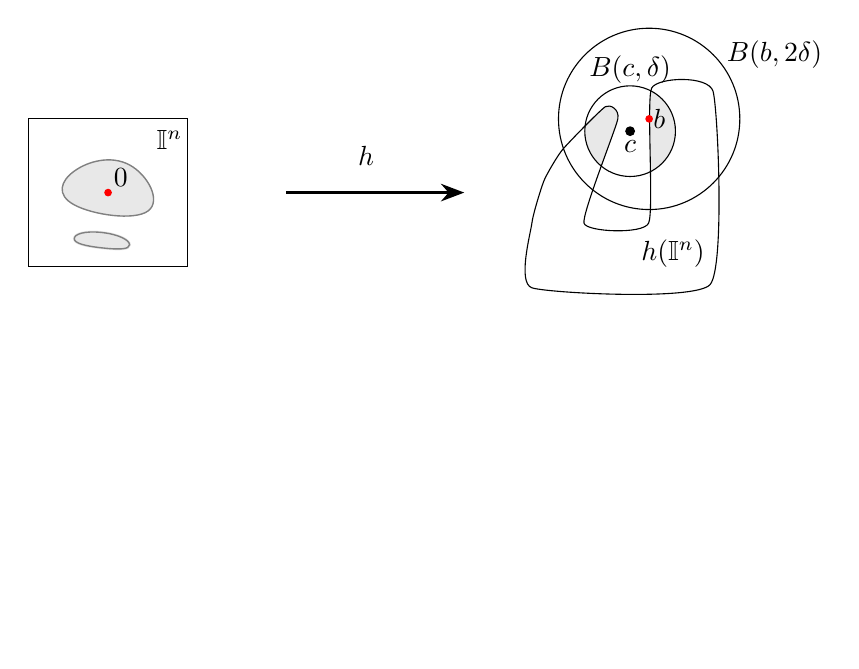
\begin{tikzpicture}[scale=0.78]
% ###############          prva slika          ###############
		\filldraw[color=gray!18] plot [smooth cycle, tension = 0.9] coordinates {(-5.15, 3.35) (-5.15, 2.8) (-3.95, 2.7) (-4.25, 3.45)};
		\draw[gray, line width=0.5pt] plot [smooth cycle, tension = 0.9] coordinates {(-5.15, 3.35) (-5.15, 2.8) (-3.95, 2.7) (-4.25, 3.45)};
		\filldraw[color=gray!18, line width=1pt] plot [smooth cycle, tension = 1.1] coordinates {(-4.25, 2.15) (-4.7, 2.35) (-5.15, 2.25) (-4.7, 2.1)};
		\draw[gray, line width=0.5pt] plot [smooth cycle, tension = 1.1] coordinates {(-4.25, 2.15) (-4.7, 2.35) (-5.15, 2.25) (-4.7, 2.1)};
		\draw (-5.9, 1.8) rectangle (-3.3, 4.2);
		\filldraw[red] (-4.6, 3) circle (1.5pt) node[black, above right=-0.7mm] {$0$};	
		 \draw (-3.6, 3.85) node {$\mathbb{I}^n$};
		
% ###############          druga slika          ###############
		\begin{scope}
			\clip plot [smooth cycle, tension = 0.3] coordinates {(2.3, 1.45) (5.2, 1.5) (5.25, 4.65) (4.25, 4.7) (4.2, 2.5) (3.15, 2.5) (3.7, 4.2) (3.5, 4.4) (2.8,3.7)  (2.5, 3.2) (2.3, 2.5)};
			\clip (3.9, 4) circle (21pt);
			\fill[color=gray!18] (-2,1.5) rectangle (6,5);
		\end{scope}
		\draw plot [smooth cycle, tension = 0.3] coordinates {(2.3, 1.45) (5.2, 1.5) (5.25, 4.65) (4.25, 4.7) (4.2, 2.5) (3.15, 2.5) (3.7, 4.2) (3.5, 4.4) (2.8,3.7)  (2.5, 3.2) (2.3, 2.5)};
		\filldraw[red] (4.21, 4.2) circle (1.5pt) node[black, right=-0.7mm] {$b$};
		\filldraw[black] (3.9, 4) circle (2pt) node[black, below =-0.1mm]{$c$};
		\draw (4.6, 2) node {$h(\mathbb{I}^n)$};
		\draw[black] (4.21, 4.2) circle (42pt);
		\draw[black] (3.9, 4) circle (21pt);
		\draw (3.9, 5) node {$B(c, \delta)$}; 
		\draw (6.25, 5.25) node {$B(b, 2 \delta)$};
	
% ###############          tretja slika          ###############
		\draw[white] (4.8, -4) node {$X$}; 
		
	% ###############          četrta slika          ###############
		
	% ###############          puščice          ###############
		\draw [black, line width=1.2pt, -Stealth] (-1.7,3) -- (1.2,3);
		\draw (-0.4, 3.6) node {$h$};
	\end{tikzpicture}
\end{figure}
\end{frame}

\begin{frame}
\frametitle{Izrek o invarianci odprtih množic}
\begin{figure}[h!]
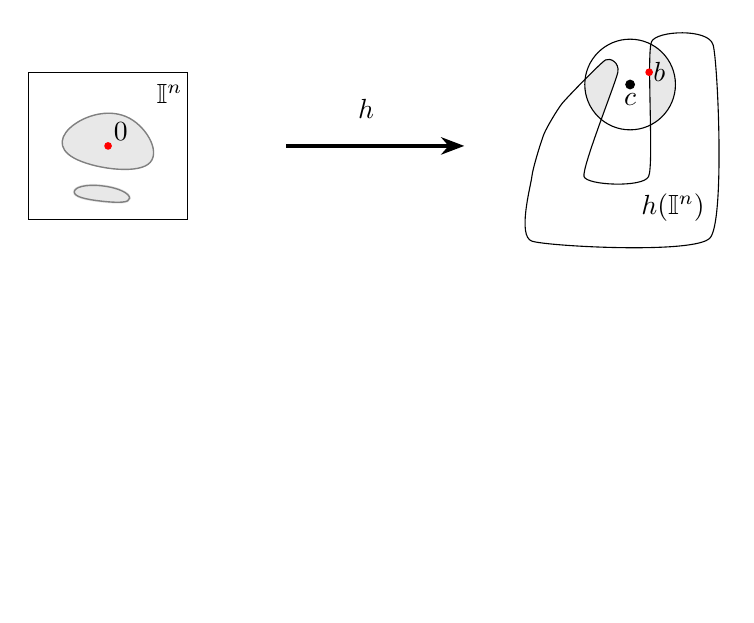
\begin{tikzpicture}[scale=0.78]
% ###############          prva slika          ###############
		\filldraw[color=gray!18] plot [smooth cycle, tension = 0.9] coordinates {(-5.15, 3.35) (-5.15, 2.8) (-3.95, 2.7) (-4.25, 3.45)};
		\draw[gray, line width=0.5pt] plot [smooth cycle, tension = 0.9] coordinates {(-5.15, 3.35) (-5.15, 2.8) (-3.95, 2.7) (-4.25, 3.45)};
		\filldraw[color=gray!18, line width=1pt] plot [smooth cycle, tension = 1.1] coordinates {(-4.25, 2.15) (-4.7, 2.35) (-5.15, 2.25) (-4.7, 2.1)};
		\draw[gray, line width=0.5pt] plot [smooth cycle, tension = 1.1] coordinates {(-4.25, 2.15) (-4.7, 2.35) (-5.15, 2.25) (-4.7, 2.1)};
		\draw (-5.9, 1.8) rectangle (-3.3, 4.2);
		\filldraw[red] (-4.6, 3) circle (1.5pt) node[black, above right=-0.7mm] {$0$};
		\draw (-4.2, 3.1) ;	
		 \draw (-3.6, 3.85) node {$\mathbb{I}^n$};
% ###############          druga slika          ###############
		\begin{scope}
			\clip plot [smooth cycle, tension = 0.3] coordinates {(2.3, 1.45) (5.2, 1.5) (5.25, 4.65) (4.25, 4.7) (4.2, 2.5) (3.15, 2.5) (3.7, 4.2) (3.5, 4.4) (2.8,3.7)  (2.5, 3.2) (2.3, 2.5)};
			\clip (3.9, 4) circle (21pt);
			\fill[color=gray!18] (-2,1.5) rectangle (6,5);
		\end{scope}
		\draw plot [smooth cycle, tension = 0.3] coordinates {(2.3, 1.45) (5.2, 1.5) (5.25, 4.65) (4.25, 4.7) (4.2, 2.5) (3.15, 2.5) (3.7, 4.2) (3.5, 4.4) (2.8,3.7)  (2.5, 3.2) (2.3, 2.5)};
		\filldraw[red] (4.21, 4.2) circle (1.5pt) node[black, right=-0.7mm] {$b$};
		\filldraw[black] (3.9, 4) circle (2pt) node[black, below =-0.1mm]{$c$};
		\draw (4.6, 2) node {$h(\mathbb{I}^n)$};
		\draw[black] (3.9, 4) circle (21pt);
	
% ###############          tretja slika          ###############
		\draw[white] (4.8, -4) node {$X$}; 
		
	% ###############          četrta slika          ###############
		
	% ###############          puščice          ###############
		\draw [black, line width=1.2pt, -Stealth] (-1.7,3) -- (1.2,3);
		\draw (-0.4, 3.6) node {$h$};
	\end{tikzpicture}
\end{figure}
\end{frame}


\begin{frame}
\frametitle{Izrek o invarianci odprtih množic}
\begin{figure}[h!]
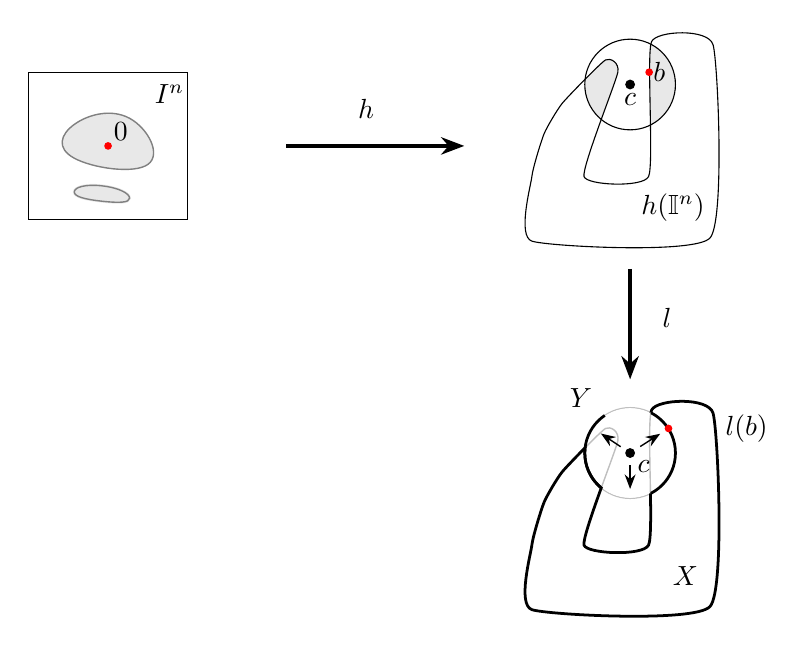
\begin{tikzpicture}[scale=0.78]
% ###############          prva slika          ###############
		\filldraw[color=gray!18] plot [smooth cycle, tension = 0.9] coordinates {(-5.15, 3.35) (-5.15, 2.8) (-3.95, 2.7) (-4.25, 3.45)};
		\draw[gray, line width=0.5pt] plot [smooth cycle, tension = 0.9] coordinates {(-5.15, 3.35) (-5.15, 2.8) (-3.95, 2.7) (-4.25, 3.45)};
		\filldraw[color=gray!18, line width=1pt] plot [smooth cycle, tension = 1.1] coordinates {(-4.25, 2.15) (-4.7, 2.35) (-5.15, 2.25) (-4.7, 2.1)};
		\draw[gray, line width=0.5pt] plot [smooth cycle, tension = 1.1] coordinates {(-4.25, 2.15) (-4.7, 2.35) (-5.15, 2.25) (-4.7, 2.1)};
		\draw (-5.9, 1.8) rectangle (-3.3, 4.2);
		\filldraw[red] (-4.6, 3) circle (1.5pt) node[black, above right=-0.7mm] {$0$};
		\draw (-4.2, 3.1) ;	
		 \draw (-3.6, 3.85) node {$I^n$};
% ###############          druga slika          ###############
		\begin{scope}
			\clip plot [smooth cycle, tension = 0.3] coordinates {(2.3, 1.45) (5.2, 1.5) (5.25, 4.65) (4.25, 4.7) (4.2, 2.5) (3.15, 2.5) (3.7, 4.2) (3.5, 4.4) (2.8,3.7)  (2.5, 3.2) (2.3, 2.5)};
			\clip (3.9, 4) circle (21pt);
			\fill[color=gray!18] (-2,1.5) rectangle (6,5);
		\end{scope}
		\draw plot [smooth cycle, tension = 0.3] coordinates {(2.3, 1.45) (5.2, 1.5) (5.25, 4.65) (4.25, 4.7) (4.2, 2.5) (3.15, 2.5) (3.7, 4.2) (3.5, 4.4) (2.8,3.7)  (2.5, 3.2) (2.3, 2.5)};
		\filldraw[red] (4.21, 4.2) circle (1.5pt) node[black, right=-0.7mm] {$b$};
		\filldraw[black] (3.9, 4) circle (2pt) node[black, below =-0.1mm]{$c$};
		\draw (4.6, 2) node {$h(\mathbb{I}^n)$};
		\draw[black] (3.9, 4) circle (21pt);
	
% ###############          tretja slika          ###############
		\draw[lightgray, line width=0.5pt] (3.9, -2) circle (21pt);
		\draw[black, line width=1pt] plot [smooth cycle, tension = 0.3] coordinates {(2.3, -4.55) (5.2, -4.5) (5.25, -1.35) (4.25, -1.3) (4.2, -3.5) (3.15, -3.5) (3.7, -1.8) (3.5, -1.6) (2.8, -2.3)  (2.5, -2.8) (2.3, -3.5)};
		\filldraw[white] (3.9, -2) circle (20.5pt);
		\begin{scope}
			\clip (3.9, -2) circle (21pt);
			\draw[lightgray, line width=0.5pt] plot [smooth cycle, tension = 0.3] coordinates {(2.3, -4.55) (5.2, -4.5) (5.25, -1.35) (4.25, -1.3) (4.2, -3.5) (3.15, -3.5) (3.7, -1.8) (3.5, -1.6) (2.8, -2.3)  (2.5, -2.8) (2.3, -3.5)};
		\end{scope}
		\begin{scope}
			\clip (3.9, -2) -- (3.4, -1.26) -- (2.5, -1) -- (3.35, -2.7) -- cycle;
			\draw[black, line width=1pt] (3.9, -2) circle (21pt);
		\end{scope}
		\begin{scope}
			\clip plot [smooth cycle, tension = 0.3] coordinates {(2.3, -4.55) (5.2, -4.5) (5.25, -1.35) (4.25, -1.3) (4.2, -3.5) (3.15, -3.5) (3.7, -1.8) (3.5, -1.6) (2.8, -2.3)  (2.5, -2.8) (2.3, -3.5)};
			\draw[black, line width=1pt] (3.9, -2) circle (21pt);
		\end{scope}
		\filldraw[black] (3.9, -2) circle (2pt) node[black, below right=-0.4mm]{$c$};
		\draw[black, line width=0.5pt, -Stealth] ($($(3.9, -2)!.5!(4.525, -1.6)$)!5pt!(3.9, -2)$) --  ($($(3.9, -2)!.5!(4.525, -1.6)$)!6pt!(4.525, -1.6)$);
		\draw[black, line width=0.5pt, -Stealth] ($($(3.9, -2)!.5!((3.9, -2.75)$)!5pt!(3.9, -2)$) --  ($($(3.9, -2)!.5!((3.9, -2.75)$)!6pt!((3.9, -2.75)$);
		\draw[black, line width=0.5pt, -Stealth] ($($(3.9, -2)!.5!(3.3, -1.6)$)!5pt!(3.9, -2)$) --  ($($(3.9, -2)!.5!(3.3, -1.6)$)!6pt!(3.3, -1.6)$);
		\filldraw[red] (4.525, -1.6) circle (1.5pt) node[black, right= 6mm] {$l(b)$};
		\draw (3.1, -1.1) node {$Y$};
		\draw (4.8, -4) node {$X$}; 
		
% ###############          četrta slika          ###############
		
% ###############          puščice          ###############
		\draw [black, line width=1.2pt, -Stealth] (-1.7,3) -- (1.2,3);
		\draw (-0.4, 3.6) node {$h$};
		\draw [black,  line width=1.2pt, -Stealth] (3.9, 1) -- (3.9, -0.8);
		\draw (4.5, 0.2) node {$l$}; 
	\end{tikzpicture}
\end{figure}
\end{frame}

\begin{frame}
\frametitle{Izrek o invarianci odprtih množic}
\begin{figure}[h!]
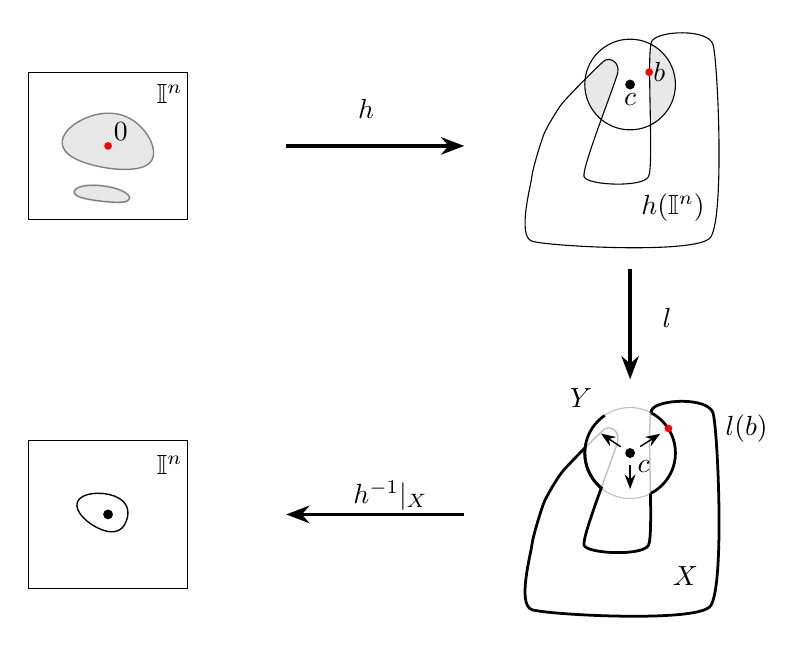
\begin{tikzpicture}[scale=0.78]
% ###############          prva slika          ###############
		\filldraw[color=gray!18] plot [smooth cycle, tension = 0.9] coordinates {(-5.15, 3.35) (-5.15, 2.8) (-3.95, 2.7) (-4.25, 3.45)};
		\draw[gray, line width=0.5pt] plot [smooth cycle, tension = 0.9] coordinates {(-5.15, 3.35) (-5.15, 2.8) (-3.95, 2.7) (-4.25, 3.45)};
		\filldraw[color=gray!18, line width=1pt] plot [smooth cycle, tension = 1.1] coordinates {(-4.25, 2.15) (-4.7, 2.35) (-5.15, 2.25) (-4.7, 2.1)};
		\draw[gray, line width=0.5pt] plot [smooth cycle, tension = 1.1] coordinates {(-4.25, 2.15) (-4.7, 2.35) (-5.15, 2.25) (-4.7, 2.1)};
		\draw (-5.9, 1.8) rectangle (-3.3, 4.2);
		\filldraw[red] (-4.6, 3) circle (1.5pt) node[black, above right=-0.7mm] {$0$};
		\draw (-4.2, 3.1) ;	
		 \draw (-3.6, 3.85) node {$\mathbb{I}^n$};
% ###############          druga slika          ###############
		\begin{scope}
			\clip plot [smooth cycle, tension = 0.3] coordinates {(2.3, 1.45) (5.2, 1.5) (5.25, 4.65) (4.25, 4.7) (4.2, 2.5) (3.15, 2.5) (3.7, 4.2) (3.5, 4.4) (2.8,3.7)  (2.5, 3.2) (2.3, 2.5)};
			\clip (3.9, 4) circle (21pt);
			\fill[color=gray!18] (-2,1.5) rectangle (6,5);
		\end{scope}
		\draw plot [smooth cycle, tension = 0.3] coordinates {(2.3, 1.45) (5.2, 1.5) (5.25, 4.65) (4.25, 4.7) (4.2, 2.5) (3.15, 2.5) (3.7, 4.2) (3.5, 4.4) (2.8,3.7)  (2.5, 3.2) (2.3, 2.5)};
		\filldraw[red] (4.21, 4.2) circle (1.5pt) node[black, right=-0.7mm] {$b$};
		\filldraw[black] (3.9, 4) circle (2pt) node[black, below =-0.1mm]{$c$};
		\draw (4.6, 2) node {$h(\mathbb{I}^n)$};
		\draw[black] (3.9, 4) circle (21pt);
	
% ###############          tretja slika          ###############
		\draw[lightgray, line width=0.5pt] (3.9, -2) circle (21pt);
		\draw[black, line width=1pt] plot [smooth cycle, tension = 0.3] coordinates {(2.3, -4.55) (5.2, -4.5) (5.25, -1.35) (4.25, -1.3) (4.2, -3.5) (3.15, -3.5) (3.7, -1.8) (3.5, -1.6) (2.8, -2.3)  (2.5, -2.8) (2.3, -3.5)};
		\filldraw[white] (3.9, -2) circle (20.5pt);
		\begin{scope}
			\clip (3.9, -2) circle (21pt);
			\draw[lightgray, line width=0.5pt] plot [smooth cycle, tension = 0.3] coordinates {(2.3, -4.55) (5.2, -4.5) (5.25, -1.35) (4.25, -1.3) (4.2, -3.5) (3.15, -3.5) (3.7, -1.8) (3.5, -1.6) (2.8, -2.3)  (2.5, -2.8) (2.3, -3.5)};
		\end{scope}
		\begin{scope}
			\clip (3.9, -2) -- (3.4, -1.26) -- (2.5, -1) -- (3.35, -2.7) -- cycle;
			\draw[black, line width=1pt] (3.9, -2) circle (21pt);
		\end{scope}
		\begin{scope}
			\clip plot [smooth cycle, tension = 0.3] coordinates {(2.3, -4.55) (5.2, -4.5) (5.25, -1.35) (4.25, -1.3) (4.2, -3.5) (3.15, -3.5) (3.7, -1.8) (3.5, -1.6) (2.8, -2.3)  (2.5, -2.8) (2.3, -3.5)};
			\draw[black, line width=1pt] (3.9, -2) circle (21pt);
		\end{scope}
		\filldraw[black] (3.9, -2) circle (2pt) node[black, below right=-0.4mm]{$c$};
		\draw[black, line width=0.5pt, -Stealth] ($($(3.9, -2)!.5!(4.525, -1.6)$)!5pt!(3.9, -2)$) --  ($($(3.9, -2)!.5!(4.525, -1.6)$)!6pt!(4.525, -1.6)$);
		\draw[black, line width=0.5pt, -Stealth] ($($(3.9, -2)!.5!((3.9, -2.75)$)!5pt!(3.9, -2)$) --  ($($(3.9, -2)!.5!((3.9, -2.75)$)!6pt!((3.9, -2.75)$);
		\draw[black, line width=0.5pt, -Stealth] ($($(3.9, -2)!.5!(3.3, -1.6)$)!5pt!(3.9, -2)$) --  ($($(3.9, -2)!.5!(3.3, -1.6)$)!6pt!(3.3, -1.6)$);
		\filldraw[red] (4.525, -1.6) circle (1.5pt) node[black, right= 6mm] {$l(b)$};
		\draw (3.1, -1.1) node {$Y$};
		\draw (4.8, -4) node {$X$}; 
		
% ###############          četrta slika          ###############
		\draw (-5.9, -4.2) rectangle (-3.3, -1.8);
		\draw[black, line width=0.5pt] plot [smooth cycle, tension = 1] coordinates {(-4.5, -2.7) (-4.3, -3.1) (-4.7, -3.25) (-5.1, -2.8)};
		\filldraw[black] (-4.6, -3) circle (2pt);
		\draw (-3.6, -2.2) node {$\mathbb{I}^n$};
% ###############          puščice          ###############
		\draw [black, line width=1.2pt, -Stealth] (-1.7,3) -- (1.2,3);
		\draw (-0.4, 3.6) node {$h$};
		\draw [black,  line width=1.2pt, -Stealth] (3.9, 1) -- (3.9, -0.8);
		\draw (4.5, 0.2) node {$l$}; 
		\draw [black,  line width=1.2pt, -Stealth] (1.2, -3) -- (-1.7, -3);
		\draw (0, -2.7) node {$h^{-1}|_{X}$};
	\end{tikzpicture}
\end{figure}
\end{frame}

\begin{frame}
\frametitle{Pomožna lema}
\begin{block}{Lema:}
Naj bo $X$ kompaktna podmnožica evklidskega prostora $\mathbb{R}^n$ in $f : X \rightarrow \mathbb{R}^n \setminus \{0\} $ zvezna preslikava. Potem za vsak $\varepsilon > 0$ in za vsako kompaktno množico s prazno notranjostjo $Y \subset \mathbb{R}^n$ obstaja zvezna preslikava $g : X \cup Y \rightarrow \mathbb{R}^n \setminus \{0\}$, da velja: $||g(x)-f(x)|| < \varepsilon$  za vsak $x \in X$
\end{block}
\end{frame}

\begin{frame}
\frametitle{Izrek o invarianci odprtih množic}
\begin{figure}[h!]
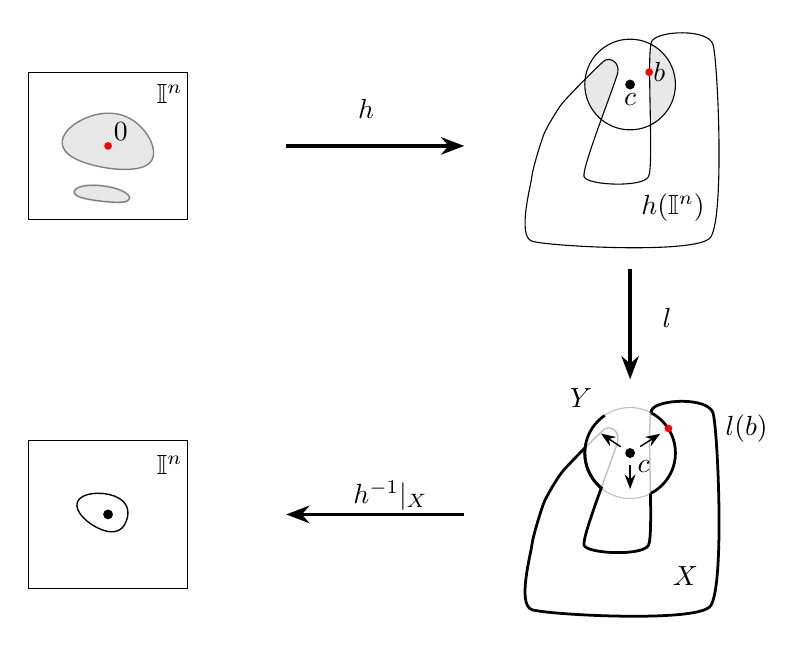
\begin{tikzpicture}[scale=0.78]
% ###############          prva slika          ###############
		\filldraw[color=gray!18] plot [smooth cycle, tension = 0.9] coordinates {(-5.15, 3.35) (-5.15, 2.8) (-3.95, 2.7) (-4.25, 3.45)};
		\draw[gray, line width=0.5pt] plot [smooth cycle, tension = 0.9] coordinates {(-5.15, 3.35) (-5.15, 2.8) (-3.95, 2.7) (-4.25, 3.45)};
		\filldraw[color=gray!18, line width=1pt] plot [smooth cycle, tension = 1.1] coordinates {(-4.25, 2.15) (-4.7, 2.35) (-5.15, 2.25) (-4.7, 2.1)};
		\draw[gray, line width=0.5pt] plot [smooth cycle, tension = 1.1] coordinates {(-4.25, 2.15) (-4.7, 2.35) (-5.15, 2.25) (-4.7, 2.1)};
		\draw (-5.9, 1.8) rectangle (-3.3, 4.2);
		\filldraw[red] (-4.6, 3) circle (1.5pt) node[black, above right=-0.7mm] {$0$};
		\draw (-4.2, 3.1) ;	
		 \draw (-3.6, 3.85) node {$\mathbb{I}^n$};
% ###############          druga slika          ###############
		\begin{scope}
			\clip plot [smooth cycle, tension = 0.3] coordinates {(2.3, 1.45) (5.2, 1.5) (5.25, 4.65) (4.25, 4.7) (4.2, 2.5) (3.15, 2.5) (3.7, 4.2) (3.5, 4.4) (2.8,3.7)  (2.5, 3.2) (2.3, 2.5)};
			\clip (3.9, 4) circle (21pt);
			\fill[color=gray!18] (-2,1.5) rectangle (6,5);
		\end{scope}
		\draw plot [smooth cycle, tension = 0.3] coordinates {(2.3, 1.45) (5.2, 1.5) (5.25, 4.65) (4.25, 4.7) (4.2, 2.5) (3.15, 2.5) (3.7, 4.2) (3.5, 4.4) (2.8,3.7)  (2.5, 3.2) (2.3, 2.5)};
		\filldraw[red] (4.21, 4.2) circle (1.5pt) node[black, right=-0.7mm] {$b$};
		\filldraw[black] (3.9, 4) circle (2pt) node[black, below =-0.1mm]{$c$};
		\draw (4.6, 2) node {$h(\mathbb{I}^n)$};
		\draw[black] (3.9, 4) circle (21pt);
	
% ###############          tretja slika          ###############
		\draw[lightgray, line width=0.5pt] (3.9, -2) circle (21pt);
		\draw[black, line width=1pt] plot [smooth cycle, tension = 0.3] coordinates {(2.3, -4.55) (5.2, -4.5) (5.25, -1.35) (4.25, -1.3) (4.2, -3.5) (3.15, -3.5) (3.7, -1.8) (3.5, -1.6) (2.8, -2.3)  (2.5, -2.8) (2.3, -3.5)};
		\filldraw[white] (3.9, -2) circle (20.5pt);
		\begin{scope}
			\clip (3.9, -2) circle (21pt);
			\draw[lightgray, line width=0.5pt] plot [smooth cycle, tension = 0.3] coordinates {(2.3, -4.55) (5.2, -4.5) (5.25, -1.35) (4.25, -1.3) (4.2, -3.5) (3.15, -3.5) (3.7, -1.8) (3.5, -1.6) (2.8, -2.3)  (2.5, -2.8) (2.3, -3.5)};
		\end{scope}
		\begin{scope}
			\clip (3.9, -2) -- (3.4, -1.26) -- (2.5, -1) -- (3.35, -2.7) -- cycle;
			\draw[black, line width=1pt] (3.9, -2) circle (21pt);
		\end{scope}
		\begin{scope}
			\clip plot [smooth cycle, tension = 0.3] coordinates {(2.3, -4.55) (5.2, -4.5) (5.25, -1.35) (4.25, -1.3) (4.2, -3.5) (3.15, -3.5) (3.7, -1.8) (3.5, -1.6) (2.8, -2.3)  (2.5, -2.8) (2.3, -3.5)};
			\draw[black, line width=1pt] (3.9, -2) circle (21pt);
		\end{scope}
		\filldraw[black] (3.9, -2) circle (2pt) node[black, below right=-0.4mm]{$c$};
		\draw[black, line width=0.5pt, -Stealth] ($($(3.9, -2)!.5!(4.525, -1.6)$)!5pt!(3.9, -2)$) --  ($($(3.9, -2)!.5!(4.525, -1.6)$)!6pt!(4.525, -1.6)$);
		\draw[black, line width=0.5pt, -Stealth] ($($(3.9, -2)!.5!((3.9, -2.75)$)!5pt!(3.9, -2)$) --  ($($(3.9, -2)!.5!((3.9, -2.75)$)!6pt!((3.9, -2.75)$);
		\draw[black, line width=0.5pt, -Stealth] ($($(3.9, -2)!.5!(3.3, -1.6)$)!5pt!(3.9, -2)$) --  ($($(3.9, -2)!.5!(3.3, -1.6)$)!6pt!(3.3, -1.6)$);
		\filldraw[red] (4.525, -1.6) circle (1.5pt) node[black, right= 6mm] {$l(b)$};
		\draw (3.1, -1.1) node {$Y$};
		\draw (4.8, -4) node {$X$}; 
		
% ###############          četrta slika          ###############
		\draw (-5.9, -4.2) rectangle (-3.3, -1.8);
		\draw[black, line width=0.5pt] plot [smooth cycle, tension = 1] coordinates {(-4.5, -2.7) (-4.3, -3.1) (-4.7, -3.25) (-5.1, -2.8)};
		\filldraw[black] (-4.6, -3) circle (2pt);
		\draw (-3.6, -2.2) node {$\mathbb{I}^n$};
% ###############          puščice          ###############
		\draw [black, line width=1.2pt, -Stealth] (-1.7,3) -- (1.2,3);
		\draw (-0.4, 3.6) node {$h$};
		\draw [black,  line width=1.2pt, -Stealth] (3.9, 1) -- (3.9, -0.8);
		\draw (4.5, 0.2) node {$l$}; 
		\draw [black,  line width=1.2pt, -Stealth] (1.2, -3) -- (-1.7, -3);
		\draw (0, -2.7) node {$h^{-1}|_{X}$};
	\end{tikzpicture}
\end{figure}
\end{frame}

\begin{frame}
\frametitle{Izrek o invarianci odprtih množic}
\begin{figure}[h!]
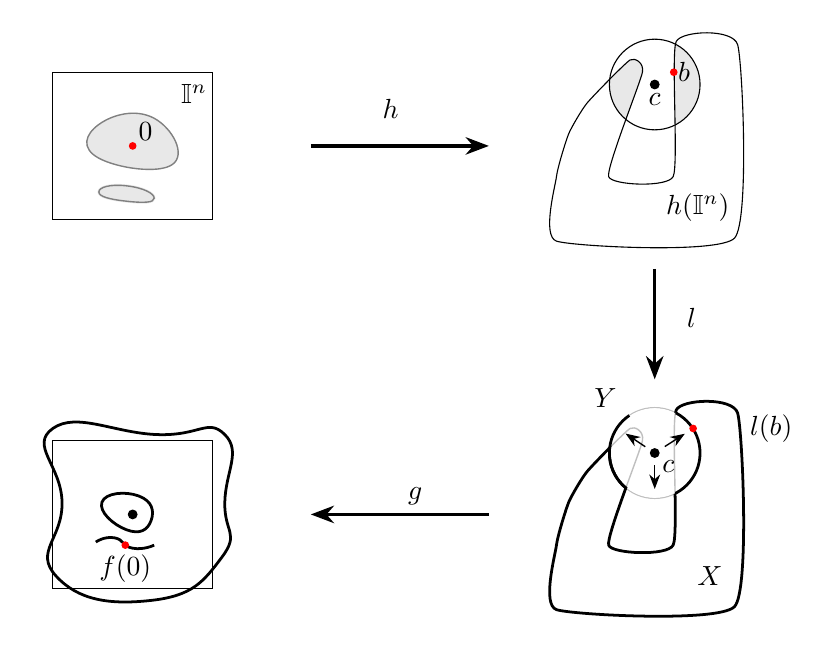
\begin{tikzpicture}[scale=0.78]
% ###############          prva slika          ###############
		\filldraw[color=gray!18] plot [smooth cycle, tension = 0.9] coordinates {(-5.15, 3.35) (-5.15, 2.8) (-3.95, 2.7) (-4.25, 3.45)};
		\draw[gray, line width=0.5pt] plot [smooth cycle, tension = 0.9] coordinates {(-5.15, 3.35) (-5.15, 2.8) (-3.95, 2.7) (-4.25, 3.45)};
		\filldraw[color=gray!18, line width=1pt] plot [smooth cycle, tension = 1.1] coordinates {(-4.25, 2.15) (-4.7, 2.35) (-5.15, 2.25) (-4.7, 2.1)};
		\draw[gray, line width=0.5pt] plot [smooth cycle, tension = 1.1] coordinates {(-4.25, 2.15) (-4.7, 2.35) (-5.15, 2.25) (-4.7, 2.1)};
		\draw (-5.9, 1.8) rectangle (-3.3, 4.2);
		\filldraw[red] (-4.6, 3) circle (1.5pt) node[black, above right=-0.7mm] {$0$};
		\draw (-4.2, 3.1) ;	
		 \draw (-3.6, 3.85) node {$\mathbb{I}^n$};
% ###############          druga slika          ###############
		\begin{scope}
			\clip plot [smooth cycle, tension = 0.3] coordinates {(2.3, 1.45) (5.2, 1.5) (5.25, 4.65) (4.25, 4.7) (4.2, 2.5) (3.15, 2.5) (3.7, 4.2) (3.5, 4.4) (2.8,3.7)  (2.5, 3.2) (2.3, 2.5)};
			\clip (3.9, 4) circle (21pt);
			\fill[color=gray!18] (-2,1.5) rectangle (6,5);
		\end{scope}
		\draw plot [smooth cycle, tension = 0.3] coordinates {(2.3, 1.45) (5.2, 1.5) (5.25, 4.65) (4.25, 4.7) (4.2, 2.5) (3.15, 2.5) (3.7, 4.2) (3.5, 4.4) (2.8,3.7)  (2.5, 3.2) (2.3, 2.5)};
		\filldraw[red] (4.21, 4.2) circle (1.5pt) node[black, right=-0.7mm] {$b$};
		\filldraw[black] (3.9, 4) circle (2pt) node[black, below =-0.1mm]{$c$};
		\draw (4.6, 2) node {$h(\mathbb{I}^n)$};
		\draw[black] (3.9, 4) circle (21pt);
	
% ###############          tretja slika          ###############
		\draw[lightgray, line width=0.5pt] (3.9, -2) circle (21pt);
		\draw[black, line width=1pt] plot [smooth cycle, tension = 0.3] coordinates {(2.3, -4.55) (5.2, -4.5) (5.25, -1.35) (4.25, -1.3) (4.2, -3.5) (3.15, -3.5) (3.7, -1.8) (3.5, -1.6) (2.8, -2.3)  (2.5, -2.8) (2.3, -3.5)};
		\filldraw[white] (3.9, -2) circle (20.5pt);
		\begin{scope}
			\clip (3.9, -2) circle (21pt);
			\draw[lightgray, line width=0.5pt] plot [smooth cycle, tension = 0.3] coordinates {(2.3, -4.55) (5.2, -4.5) (5.25, -1.35) (4.25, -1.3) (4.2, -3.5) (3.15, -3.5) (3.7, -1.8) (3.5, -1.6) (2.8, -2.3)  (2.5, -2.8) (2.3, -3.5)};
		\end{scope}
		\begin{scope}
			\clip (3.9, -2) -- (3.4, -1.26) -- (2.5, -1) -- (3.35, -2.7) -- cycle;
			\draw[black, line width=1pt] (3.9, -2) circle (21pt);
		\end{scope}
		\begin{scope}
			\clip plot [smooth cycle, tension = 0.3] coordinates {(2.3, -4.55) (5.2, -4.5) (5.25, -1.35) (4.25, -1.3) (4.2, -3.5) (3.15, -3.5) (3.7, -1.8) (3.5, -1.6) (2.8, -2.3)  (2.5, -2.8) (2.3, -3.5)};
			\draw[black, line width=1pt] (3.9, -2) circle (21pt);
		\end{scope}
		\filldraw[black] (3.9, -2) circle (2pt) node[black, below right=-0.4mm]{$c$};
		\draw[black, line width=0.5pt, -Stealth] ($($(3.9, -2)!.5!(4.525, -1.6)$)!5pt!(3.9, -2)$) --  ($($(3.9, -2)!.5!(4.525, -1.6)$)!6pt!(4.525, -1.6)$);
		\draw[black, line width=0.5pt, -Stealth] ($($(3.9, -2)!.5!((3.9, -2.75)$)!5pt!(3.9, -2)$) --  ($($(3.9, -2)!.5!((3.9, -2.75)$)!6pt!((3.9, -2.75)$);
		\draw[black, line width=0.5pt, -Stealth] ($($(3.9, -2)!.5!(3.3, -1.6)$)!5pt!(3.9, -2)$) --  ($($(3.9, -2)!.5!(3.3, -1.6)$)!6pt!(3.3, -1.6)$);
		\filldraw[red] (4.525, -1.6) circle (1.5pt) node[black, right= 6mm] {$l(b)$};
		\draw (3.1, -1.1) node {$Y$};
		\draw (4.8, -4) node {$X$}; 
		
% ###############          četrta slika          ###############
		\draw (-5.9, -4.2) rectangle (-3.3, -1.8);
		\draw[black, line width=1pt] plot [smooth cycle, tension = 1] coordinates {(-4.5, -2.7) (-4.3, -3.1) (-4.7, -3.25) (-5.1, -2.8)};
		\draw[black, line width=1pt] plot [smooth, tension = 1] coordinates {(-5.2, -3.45) (-4.9, -3.38) (-4.6, -3.55) (-4.25, -3.5)};
		\filldraw[red] (-4.72, -3.5) circle (1.5pt) node[black, below] {$f(0)$};
		\filldraw[black] (-4.6, -3) circle (2pt);
		\draw[black, line width=1pt] plot [smooth cycle, tension = 0.9] coordinates { (-3.1, -1.7) (-4.2, -1.7) (-5.9, -1.6) (-5.75, -2.8) (-5.85, -4) (-4.3, -4.4) (-3.15, -3.7) (-3.1, -2.8)};
% ###############          puščice          ###############
		\draw [black, line width=1.2pt, -Stealth] (-1.7,3) -- (1.2,3);
		\draw (-0.4, 3.6) node {$h$};
		\draw [black,  line width=1.2pt, -Stealth] (3.9, 1) -- (3.9, -0.8);
		\draw (4.5, 0.2) node {$l$}; 
		\draw [black,  line width=1.2pt, -Stealth] (1.2, -3) -- (-1.7, -3);
		\draw (0, -2.7) node {$g$};
	\end{tikzpicture}
\end{figure}
\end{frame}

\begin{frame}
\frametitle{Izrek o invarianci odprtih množic}
\begin{figure}[h!]
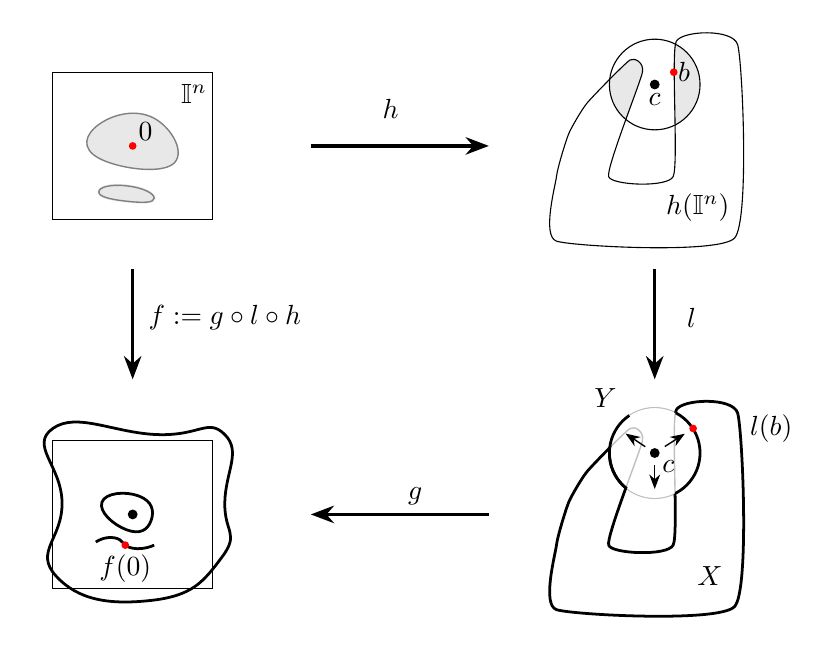
\begin{tikzpicture}[scale=0.78]
% ###############          prva slika          ###############
		\filldraw[color=gray!18] plot [smooth cycle, tension = 0.9] coordinates {(-5.15, 3.35) (-5.15, 2.8) (-3.95, 2.7) (-4.25, 3.45)};
		\draw[gray, line width=0.5pt] plot [smooth cycle, tension = 0.9] coordinates {(-5.15, 3.35) (-5.15, 2.8) (-3.95, 2.7) (-4.25, 3.45)};
		\filldraw[color=gray!18, line width=1pt] plot [smooth cycle, tension = 1.1] coordinates {(-4.25, 2.15) (-4.7, 2.35) (-5.15, 2.25) (-4.7, 2.1)};
		\draw[gray, line width=0.5pt] plot [smooth cycle, tension = 1.1] coordinates {(-4.25, 2.15) (-4.7, 2.35) (-5.15, 2.25) (-4.7, 2.1)};
		\draw (-5.9, 1.8) rectangle (-3.3, 4.2);
		\filldraw[red] (-4.6, 3) circle (1.5pt) node[black, above right=-0.7mm] {$0$};
		\draw (-4.2, 3.1) ;	
		 \draw (-3.6, 3.85) node {$\mathbb{I}^n$};
		
% ###############          druga slika          ###############
		\begin{scope}
			\clip plot [smooth cycle, tension = 0.3] coordinates {(2.3, 1.45) (5.2, 1.5) (5.25, 4.65) (4.25, 4.7) (4.2, 2.5) (3.15, 2.5) (3.7, 4.2) (3.5, 4.4) (2.8,3.7)  (2.5, 3.2) (2.3, 2.5)};
			\clip (3.9, 4) circle (21pt);
			\fill[color=gray!18] (-2,1.5) rectangle (6,5);
		\end{scope}
		\draw plot [smooth cycle, tension = 0.3] coordinates {(2.3, 1.45) (5.2, 1.5) (5.25, 4.65) (4.25, 4.7) (4.2, 2.5) (3.15, 2.5) (3.7, 4.2) (3.5, 4.4) (2.8,3.7)  (2.5, 3.2) (2.3, 2.5)};
		\filldraw[black] (3.9, 4) circle (2pt) node[black, below =-0.1mm]{$c$};
		\filldraw[red] (4.21, 4.2) circle (1.5pt) node[black, right=-0.7mm] {$b$};
		\draw[black] (3.9, 4) circle (21pt);
		\draw (4.6, 2) node {$h(\mathbb{I}^n)$};
	
% ###############          tretja slika          ###############
		\draw[lightgray, line width=0.5pt] (3.9, -2) circle (21pt);
		\draw[black, line width=1pt] plot [smooth cycle, tension = 0.3] coordinates {(2.3, -4.55) (5.2, -4.5) (5.25, -1.35) (4.25, -1.3) (4.2, -3.5) (3.15, -3.5) (3.7, -1.8) (3.5, -1.6) (2.8, -2.3)  (2.5, -2.8) (2.3, -3.5)};
		\filldraw[white] (3.9, -2) circle (20.5pt);
		\begin{scope}
			\clip (3.9, -2) circle (21pt);
			\draw[lightgray, line width=0.5pt] plot [smooth cycle, tension = 0.3] coordinates {(2.3, -4.55) (5.2, -4.5) (5.25, -1.35) (4.25, -1.3) (4.2, -3.5) (3.15, -3.5) (3.7, -1.8) (3.5, -1.6) (2.8, -2.3)  (2.5, -2.8) (2.3, -3.5)};
		\end{scope}
		\begin{scope}
			\clip (3.9, -2) -- (3.4, -1.26) -- (2.5, -1) -- (3.35, -2.7) -- cycle;
			\draw[black, line width=1pt] (3.9, -2) circle (21pt);
		\end{scope}
		\begin{scope}
			\clip plot [smooth cycle, tension = 0.3] coordinates {(2.3, -4.55) (5.2, -4.5) (5.25, -1.35) (4.25, -1.3) (4.2, -3.5) (3.15, -3.5) (3.7, -1.8) (3.5, -1.6) (2.8, -2.3)  (2.5, -2.8) (2.3, -3.5)};
			\draw[black, line width=1pt] (3.9, -2) circle (21pt);
		\end{scope}
		\filldraw[black] (3.9, -2) circle (2pt) node[black, below right=-0.4mm]{$c$};
		\draw[black, line width=0.5pt, -Stealth] ($($(3.9, -2)!.5!(4.525, -1.6)$)!5pt!(3.9, -2)$) --  ($($(3.9, -2)!.5!(4.525, -1.6)$)!6pt!(4.525, -1.6)$);
		\draw[black, line width=0.5pt, -Stealth] ($($(3.9, -2)!.5!((3.9, -2.75)$)!5pt!(3.9, -2)$) --  ($($(3.9, -2)!.5!((3.9, -2.75)$)!6pt!((3.9, -2.75)$);
		\draw[black, line width=0.5pt, -Stealth] ($($(3.9, -2)!.5!(3.3, -1.6)$)!5pt!(3.9, -2)$) --  ($($(3.9, -2)!.5!(3.3, -1.6)$)!6pt!(3.3, -1.6)$);
		\filldraw[red] (4.525, -1.6) circle (1.5pt) node[black, right= 6mm] {$l(b)$};
		\draw (3.1, -1.1) node {$Y$};
		\draw (4.8, -4) node {$X$}; 
		
	% ###############          četrta slika          ###############
		\draw (-5.9, -4.2) rectangle (-3.3, -1.8);
		\draw[black, line width=1pt] plot [smooth cycle, tension = 1] coordinates {(-4.5, -2.7) (-4.3, -3.1) (-4.7, -3.25) (-5.1, -2.8)};
		\draw[black, line width=1pt] plot [smooth, tension = 1] coordinates {(-5.2, -3.45) (-4.9, -3.38) (-4.6, -3.55) (-4.25, -3.5)};
		\filldraw[red] (-4.72, -3.5) circle (1.5pt) node[black, below] {$f(0)$};
		\filldraw[black] (-4.6, -3) circle (2pt);
		\draw[black, line width=1pt] plot [smooth cycle, tension = 0.9] coordinates { (-3.1, -1.7) (-4.2, -1.7) (-5.9, -1.6) (-5.75, -2.8) (-5.85, -4) (-4.3, -4.4) (-3.15, -3.7) (-3.1, -2.8)};
	
	% ###############          puščice          ###############
		\draw [black, line width=1.2pt, -Stealth] (-1.7,3) -- (1.2,3);
		\draw (-0.4, 3.6) node {$h$};
		\draw [black,  line width=1.2pt, -Stealth] (1.2, -3) -- (-1.7, -3);
		\draw (0, -2.7) node {$g$};
		\draw [black,  line width=1.2pt, -Stealth] (-4.6, 1) -- (-4.6, -0.8);
		\draw (-3.1, 0.2) node {$f  := g \circ l \circ h$};
		\draw [black,  line width=1.2pt, -Stealth] (3.9, 1) -- (3.9, -0.8);
		\draw (4.5, 0.2) node {$l$};  
	\end{tikzpicture}
\end{figure}
\end{frame}

\begin{frame}
\frametitle{Poincar\'{e}-Mirandov izrek}
% Vsebina prosojnice 1
\begin{block}{Definicija:}
Naj bo število $a>0$.
Za kocko $\mathbb{I}^n = [-a, a]^n$ definiramo:
\begin{itemize}
\item $\mathbb{I}_i ^- =\{(x_1, x_2, \dots, x_n) \in \mathbb{I}^n | x_i = -a\}$ in
\item $\mathbb{I}_i ^+ =\{(x_1, x_2, \dots, x_n) \in \mathbb{I}^n | x_i = a\}$
\end{itemize}
\end{block}

\begin{figure}
\includegraphics[width=9cm]{poincare_oznake.pdf}
\end{figure}
\end{frame}


\begin{frame}
\frametitle{Poincar\'{e}-Mirandov izrek}
\begin{block}{Poincar\'{e}-Mirandov izrek:}
Naj bo $f = (f_1, f_2, \dots, f_n) : \mathbb{I}^n \rightarrow \mathbb{R}^n$ taka zvezna preslikava, da je 
\begin{itemize}
\item $f_i (\mathbb{I}_i ^-) \subset (-\infty, 0]$ in
\item $f_i (\mathbb{I}_i ^+) \subset [0, \infty)$, za vsak $i \in (1, \dots, n)$.
\end{itemize}
Potem obstaja točka $z\in \mathbb{I}^n$, da je $f(z) = 0$.
\end{block}
\end{frame}

\begin{frame}
\frametitle{Izrek o invarianci odprtih množic}
\begin{figure}[h!]
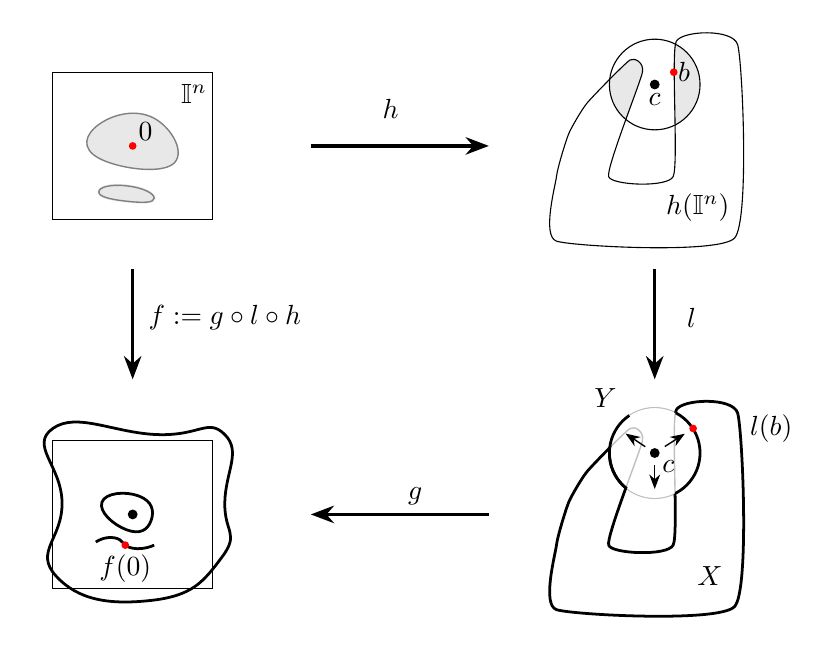
\begin{tikzpicture}[scale=0.78]
% ###############          prva slika          ###############
		\filldraw[color=gray!18] plot [smooth cycle, tension = 0.9] coordinates {(-5.15, 3.35) (-5.15, 2.8) (-3.95, 2.7) (-4.25, 3.45)};
		\draw[gray, line width=0.5pt] plot [smooth cycle, tension = 0.9] coordinates {(-5.15, 3.35) (-5.15, 2.8) (-3.95, 2.7) (-4.25, 3.45)};
		\filldraw[color=gray!18, line width=1pt] plot [smooth cycle, tension = 1.1] coordinates {(-4.25, 2.15) (-4.7, 2.35) (-5.15, 2.25) (-4.7, 2.1)};
		\draw[gray, line width=0.5pt] plot [smooth cycle, tension = 1.1] coordinates {(-4.25, 2.15) (-4.7, 2.35) (-5.15, 2.25) (-4.7, 2.1)};
		\draw (-5.9, 1.8) rectangle (-3.3, 4.2);
		\filldraw[red] (-4.6, 3) circle (1.5pt) node[black, above right=-0.7mm] {$0$};
		\draw (-4.2, 3.1) ;	
		 \draw (-3.6, 3.85) node {$\mathbb{I}^n$};
		
% ###############          druga slika          ###############
		\begin{scope}
			\clip plot [smooth cycle, tension = 0.3] coordinates {(2.3, 1.45) (5.2, 1.5) (5.25, 4.65) (4.25, 4.7) (4.2, 2.5) (3.15, 2.5) (3.7, 4.2) (3.5, 4.4) (2.8,3.7)  (2.5, 3.2) (2.3, 2.5)};
			\clip (3.9, 4) circle (21pt);
			\fill[color=gray!18] (-2,1.5) rectangle (6,5);
		\end{scope}
		\draw plot [smooth cycle, tension = 0.3] coordinates {(2.3, 1.45) (5.2, 1.5) (5.25, 4.65) (4.25, 4.7) (4.2, 2.5) (3.15, 2.5) (3.7, 4.2) (3.5, 4.4) (2.8,3.7)  (2.5, 3.2) (2.3, 2.5)};
		\filldraw[black] (3.9, 4) circle (2pt) node[black, below =-0.1mm]{$c$};
		\filldraw[red] (4.21, 4.2) circle (1.5pt) node[black, right=-0.7mm] {$b$};
		\draw[black] (3.9, 4) circle (21pt);
		\draw (4.6, 2) node {$h(\mathbb{I}^n)$};
	
% ###############          tretja slika          ###############
		\draw[lightgray, line width=0.5pt] (3.9, -2) circle (21pt);
		\draw[black, line width=1pt] plot [smooth cycle, tension = 0.3] coordinates {(2.3, -4.55) (5.2, -4.5) (5.25, -1.35) (4.25, -1.3) (4.2, -3.5) (3.15, -3.5) (3.7, -1.8) (3.5, -1.6) (2.8, -2.3)  (2.5, -2.8) (2.3, -3.5)};
		\filldraw[white] (3.9, -2) circle (20.5pt);
		\begin{scope}
			\clip (3.9, -2) circle (21pt);
			\draw[lightgray, line width=0.5pt] plot [smooth cycle, tension = 0.3] coordinates {(2.3, -4.55) (5.2, -4.5) (5.25, -1.35) (4.25, -1.3) (4.2, -3.5) (3.15, -3.5) (3.7, -1.8) (3.5, -1.6) (2.8, -2.3)  (2.5, -2.8) (2.3, -3.5)};
		\end{scope}
		\begin{scope}
			\clip (3.9, -2) -- (3.4, -1.26) -- (2.5, -1) -- (3.35, -2.7) -- cycle;
			\draw[black, line width=1pt] (3.9, -2) circle (21pt);
		\end{scope}
		\begin{scope}
			\clip plot [smooth cycle, tension = 0.3] coordinates {(2.3, -4.55) (5.2, -4.5) (5.25, -1.35) (4.25, -1.3) (4.2, -3.5) (3.15, -3.5) (3.7, -1.8) (3.5, -1.6) (2.8, -2.3)  (2.5, -2.8) (2.3, -3.5)};
			\draw[black, line width=1pt] (3.9, -2) circle (21pt);
		\end{scope}
		\filldraw[black] (3.9, -2) circle (2pt) node[black, below right=-0.4mm]{$c$};
		\draw[black, line width=0.5pt, -Stealth] ($($(3.9, -2)!.5!(4.525, -1.6)$)!5pt!(3.9, -2)$) --  ($($(3.9, -2)!.5!(4.525, -1.6)$)!6pt!(4.525, -1.6)$);
		\draw[black, line width=0.5pt, -Stealth] ($($(3.9, -2)!.5!((3.9, -2.75)$)!5pt!(3.9, -2)$) --  ($($(3.9, -2)!.5!((3.9, -2.75)$)!6pt!((3.9, -2.75)$);
		\draw[black, line width=0.5pt, -Stealth] ($($(3.9, -2)!.5!(3.3, -1.6)$)!5pt!(3.9, -2)$) --  ($($(3.9, -2)!.5!(3.3, -1.6)$)!6pt!(3.3, -1.6)$);
		\filldraw[red] (4.525, -1.6) circle (1.5pt) node[black, right= 6mm] {$l(b)$};
		\draw (3.1, -1.1) node {$Y$};
		\draw (4.8, -4) node {$X$}; 
		
	% ###############          četrta slika          ###############
		\draw (-5.9, -4.2) rectangle (-3.3, -1.8);
		\draw[black, line width=1pt] plot [smooth cycle, tension = 1] coordinates {(-4.5, -2.7) (-4.3, -3.1) (-4.7, -3.25) (-5.1, -2.8)};
		\draw[black, line width=1pt] plot [smooth, tension = 1] coordinates {(-5.2, -3.45) (-4.9, -3.38) (-4.6, -3.55) (-4.25, -3.5)};
		\filldraw[red] (-4.72, -3.5) circle (1.5pt) node[black, below] {$f(0)$};
		\filldraw[black] (-4.6, -3) circle (2pt);
		\draw[black, line width=1pt] plot [smooth cycle, tension = 0.9] coordinates { (-3.1, -1.7) (-4.2, -1.7) (-5.9, -1.6) (-5.75, -2.8) (-5.85, -4) (-4.3, -4.4) (-3.15, -3.7) (-3.1, -2.8)};
	
	% ###############          puščice          ###############
		\draw [black, line width=1.2pt, -Stealth] (-1.7,3) -- (1.2,3);
		\draw (-0.4, 3.6) node {$h$};
		\draw [black,  line width=1.2pt, -Stealth] (1.2, -3) -- (-1.7, -3);
		\draw (0, -2.7) node {$g$};
		\draw [black,  line width=1.2pt, -Stealth] (-4.6, 1) -- (-4.6, -0.8);
		\draw (-3.1, 0.2) node {$f  := g \circ l \circ h$};
		\draw [black,  line width=1.2pt, -Stealth] (3.9, 1) -- (3.9, -0.8);
		\draw (4.5, 0.2) node {$l$};  
	\end{tikzpicture}
\end{figure}
\end{frame}



\begin{frame}
\frametitle{Poincar\'{e}-Mirandov izrek}
\begin{block}{Poincar\'{e}-Mirandov izrek:}
Naj bo $f = (f_1, f_2, \dots, f_n) : \mathbb{I}^n \rightarrow \mathbb{R}^n$ taka zvezna preslikava, da je 
\begin{itemize}
\item $f_i (\mathbb{I}_i ^-) \subset (-\infty, 0]$ in
\item $f_i (\mathbb{I}_i ^+) \subset [0, \infty)$, za vsak $i \in (1, \dots, n)$.
\end{itemize}
Potem obstaja točka $x\in \mathbb{I}^n$, da je $f(x) = 0$.
\end{block}
\end{frame}

\begin{frame}
\frametitle{Izrek o vmesni vrednosti}
% Vsebina prosojnice 1

\begin{figure}
\includegraphics[width=9cm]{bolzano.pdf}
\end{figure}
\end{frame}

\begin{frame}
\frametitle{Poincar\'{e}  Mirandov izrek v dveh dimenzijah}
% Vsebina prosojnice 1

\begin{center}
\definecolor{qqqqff}{rgb}{0.,0.,1.}
\definecolor{qqffqq}{rgb}{0.,1.,0.}
\definecolor{ffqqqq}{rgb}{1.,0.,0.}
\begin{tikzpicture}[line cap=round,line join=round,>=triangle 45,x=3cm,y=2.8cm]
\draw[->,color=black] (-1.2989699661422938,0.) -- (1.3004294446621418,0.);
\foreach \x in {-1.,1.}
\draw[shift={(\x,0)},color=black] (0pt,2pt) -- (0pt,-2pt) node[anchor=north west] {\footnotesize $\x$};
\draw[->,color=black] (0.,-1.1997342918318246) -- (0.,1.2003342741882355);
\foreach \y in {-1.,1.}
\draw[shift={(0,\y)},color=black] (2pt,0pt) -- (-2pt,0pt) node[anchor=south east] {\footnotesize $\y$};
\draw[color=black] (0pt,-10pt) node[right] {\footnotesize $0$};
\clip(-1.2989699661422938,-1.1997342918318246) rectangle (1.3004294446621418,1.2003342741882355);
\fill[line width=0.pt,color=ffqqqq,fill=ffqqqq,fill opacity=0.05000000074505806] (-1.,-1.) -- (1.,-1.) -- (1.,1.) -- (-1.,1.) -- cycle;
\draw [line width=1.2pt,color=ffqqqq] (-1.,1.)-- (1.,1.);
\draw [line width=1.2pt,color=ffqqqq] (-1.,-1.)-- (1.,-1.);
\draw [line width=1.2pt,color=qqffqq] (-1.,-1.)-- (-1.,1.);
\draw [line width=1.2pt,color=qqffqq] (1.,-1.)-- (1.,1.);
\draw [line width=1.6pt,color=ffqqqq] (-1.,0.7378784755666599)-- (0.16559573064227023,0.45675274843267155);
\draw [line width=1.6pt,color=ffqqqq] (0.16559573064227023,0.45675274843267155)-- (0.41504531950764095,-0.461855261357262);
\draw [line width=1.6pt,color=ffqqqq] (0.41504531950764095,-0.461855261357262)-- (1.,-0.8);
\draw [line width=1.6pt,color=qqffqq] (-0.5352388285509141,1.)-- (-0.3887366890585536,0.10435571019429186);
\draw [line width=1.6pt,color=qqffqq] (-0.3887366890585536,0.10435571019429186)-- (0.403166767656909,-0.6835882292375908);
\draw [line width=1.6pt,color=qqffqq] (0.403166767656909,-0.6835882292375908)-- (0.529871320731383,-1.);
\draw [line width=2.pt,color=qqqqff] (-0.4715136823191907,0.6104148134815943) circle (0.1cm);
\draw (-1,1.2) node[anchor=north west] {\textbf{$f=(f_1, f_2)$}};
\draw (-1.25,0.2) node[anchor=north west] {\textbf{$f_1<0$}};
\draw (0.75,0.2) node[anchor=north west] {\textbf{$f_1>0$}};
\draw (0.07480588827248567,1.2) node[anchor=north west] {\textbf{$f_2>0$}};
\draw (0.069418531980663,-1.) node[anchor=north west] {\textbf{$f_2<0$}};
\draw (0.2,0.4) node[anchor=north west] {\textbf{$f_2 = 0$}};
\draw (-0.5716768667462341,-0.1) node[anchor=north west] {\textbf{$f_1 = 0$}};
\begin{scriptsize}
\draw [fill=black] (-1.,1.) circle (1.5pt);
\draw [fill=black] (1.,1.) circle (1.5pt);
\draw [fill=black] (-1.,-1.) circle (1.5pt);
\draw [fill=black] (1.,-1.) circle (1.5pt);
\draw [fill=qqqqff] (-0.4715136823191907,0.6104148134815943) circle (1.5pt);
\end{scriptsize}
\end{tikzpicture}
\end{center}
\end{frame}

\begin{frame}
\frametitle{Dokazovanje Poincar\'{e}  Mirandovega izreka}
\begin{figure}
\includegraphics[width=7cm]{sosed.pdf}
\end{figure}
\end{frame}

\begin{frame}
\frametitle{Dokazovanje Poincar\'{e}  Mirandovega izreka}
\begin{figure}
\includegraphics[width=7cm]{konvergenca.pdf}
\end{figure}
\end{frame}

\begin{frame}
\frametitle{Spernerjeva lema}
\begin{figure}
\includegraphics[width=8.5cm]{spernerjevo_barvanje.pdf}
\end{figure}
\end{frame}

\end{document}
